\documentclass[]{IEEEtran}

\title{Integrazione su Virtual Platform e modellazione con SystemC-TLM di un Moltiplicatore Floating-point Single Precision}
\author{Enrico Sgarbanti - VR446095}

\usepackage{graphicx}
\usepackage{subfig}
\usepackage{wrapfig}
\usepackage{hyperref}
\usepackage[italian]{babel}
\usepackage[utf8]{inputenc}

\begin{document}
\maketitle



\begin{abstract}
    Questo documento mostra l'integrazione di un modulo, che realizza due moltiplicazioni a virgola mobile singola precisione secondo lo standard IEEE754\cite{IEEE754}, nella virtual platform COM6502-Splatters e sua modellazione in SystemC\cite{SystemC} TLM nei diversi stili.
\end{abstract}



\section{Introduzione}
Il primo obiettivo consiste nell'integrare nella virtual platform COM6502-Splatters il modulo double\_multiplier creato nel primo progetto. L'idea è fare un piccolo software da caricare nella ROM che richiede l'esecuzione di due moltiplicazioni con quattro operandi, scelti arbitrariamente, di cui uno letto da input. Per fare ciò, utilizzando il protocllo AMBA APB, è necessario realizzare un wrapper del double\_multiplier per collegare il componente al bus e un driver per farsì che esso possa essere invocato dal software.
\\Il secondo obiettivo è implementare il componente double\_multiplier nei vari stili di SystemC-TLM e fare con confronto con l'implementazione in SystemC-RTL. Ci si aspetta che con l'aumentare dell'accuratezza della descrizione temporale, la simulazione richiederà più tempo.



\section{Background}
Nel classico flusso di progettazione di un sistema embedded si parte a sviluppare software solo dopo aver finito la progettazione hardware. Manca però una visione concretamente utilizzabile all'interno del sistema, prima della fase di tape-out, e ciò porta spesso a dover modificare il codice, aumentando così il time-to-market.
La \textbf{progettazione basata su piattaforma} è la creazione di un'architettura stabile basata su microprocessore che può essere rapidamente estesa, personalizzata per diverse applicazioni e consegnata ai clienti per una rapida implementazione. (J.M. Chateau-STMicroelectornics). Essa permette di fare verifica funzionale, stime di tempo per analisi di perfomance, partizionare hardware e software, porta ad un incremento della velocità e permette modularità e riuso.
\\La modellazione a livello di transazione (\textbf{TLM}) è un tipo di progettazione che sta tra il livello algoritmico e quello RT. I dettagli di implementazione vengono astratti preservando però gli aspetti comportamentali del sistema, permettendo quindi una simulazione più veloce, ma meno accurata di quella RTL. Fornisce quindi una piattaforma dove si può iniziare rapidamente a sviluppare software, molto prima rispetto al classico flusso di sviluppo.
\\In SystemC-TLM la comunicazione tra componenti si ottiene dallo scambio di pacchetti tra un modulo \textbf{initiator} e un modulo \textbf{target} attraverso 0 o più componenti intermedi. Il trasferimento di dati da un modulo ad un altro è detto \textbf{transazione} e avviene attraverso una \textbf{socket}. Il percorso che compiono i dati dal initiator al target è detto \textbf{forward-path}, invece quello dal target all'initiator è detto \textbf{backward-path} e lo si utilizza solo se l'interfaccia è non bloccante. Ci sono tre principali stili che definiscono la relazione tra tempo e dati e permettono al progettista di descrivere il sistema con livello più o meno astratto:
\begin{itemize}
    \item \textbf{Approximately timed: } le transazioni sono divise in quattro fasi: inizio richiesta, fine richiesta, inizio risposta, fine risposta. L'interfaccia è non bloccante quindi viene usato sia il forward-path che il backward-path. Esso è indicato per l'esplorazione architetturale e l'analisi delle performance.
    \item \textbf{Loosely timed: } le transazioni sono divise in due fasi: inizio transizione, fine transizione. L'interfaccia è bloccante quindi viene usato solo il forward-path poichè l'initiator aspetta la risposta del target. Esso rappresenta i dettagli di temporizzazione sufficienti per avviare un sistema operativo ed eseguire sistemi multi-core.
    \item \textbf{Untimed: } la nozione di tempo non è necessaria e quindi non viene presa in considerazione.
\end{itemize}

\begin{figure}[!htb]
    \centering
    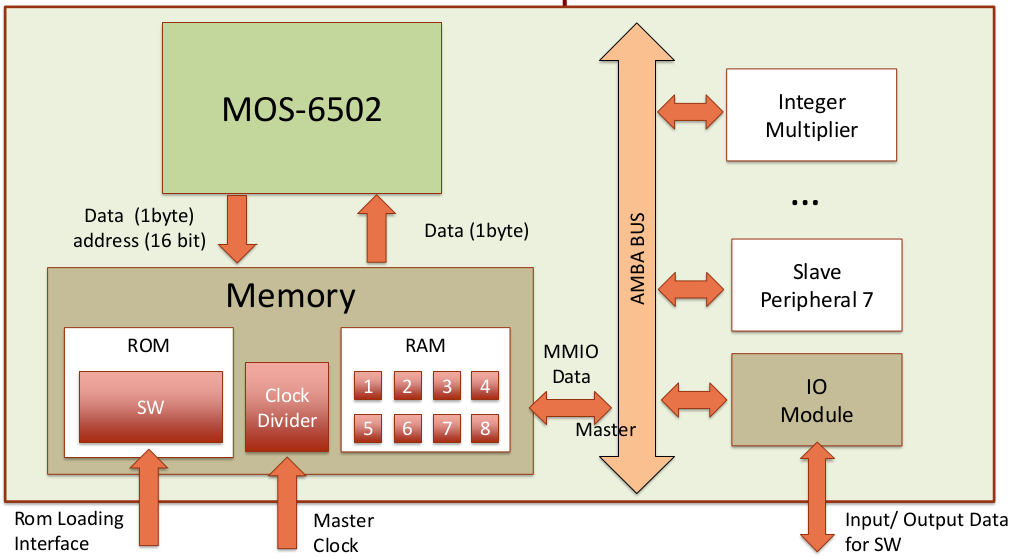
\includegraphics[width=0.9\linewidth]{figures/splatters}
    \caption{COM6502-Splatters}
    \label{fig:splatters}
\end{figure}
La virtual platform utilizzata è COM6502-Splatters [Figura \ref{fig:splatters}] che include:
\begin{itemize}
    \item \textbf{CPU} MOS 6502 (1975) con indirizzamento a 16 bit e gestione di dati in 8 bit.
    \item \textbf{ROM} da 16KB in un singolo blocco.
    \item \textbf{RAM} da 16KB divisa in 8 blocchi per permettere operazioni multiple di lettura/scrittura.
    \item \textbf{BUS} ARM APB (advanced peripherical Bus) che supporta fino a 8 periferiche.
    \item \textbf{IO Module} usato per richiedere e inviare dati alla piattaforma.
    \item \textbf{Multiplier} usato per eseguire moltiplicazioni fra interi.
\end{itemize}
Essa deve essere compilata col cross-compilatore cc65\cite{CC65}.
\\\textbf{MBA} (Advanced Microcontroller Bus Architecture) è uno standard open-source di ARM per la connessione e la gestione di blocchi funzionali nei progetti di system-on-a-chip. Nella versione APB (Advanced peripherical bus) ci sono due attori: \textbf{Master} che controlla le perifiriche; \textbf{Slave} periferica controllata dal master. I segnali utilizzati in questo protocollo sono:
\begin{itemize}
    \item \textbf{pclk:} segnale di clock della periferica.
    \item \textbf{preset:} segnale di reset della periferica.
    \item \textbf{paddr:} indirizzo.
    \item \textbf{psel:} segnale che indica se la periferica è stata selezionata.
    \item \textbf{penable:} segnale che indica se la periferica è stata abilitata.
    \item \textbf{pwrite:} segnale che indica operazioni di scrittura (1) o lettura (0) sulla periferica.
    \item \textbf{pwdata:} dati sulla periferica da parte del Master.
    \item \textbf{pready:} segnale che indica che i dati per il Master sono pronti.
    \item \textbf{prdata:} dati sulla periferica per il Master.
\end{itemize}



\section{Metodologia applicata}

\subsection{Struttura progetto}
\begin{itemize}
    \item \textbf{Virtual\_Platform/}
          \begin{itemize}
              \item \textbf{application/} cartella contenente il codice sorgente dell'software e dei driver.
              \item \textbf{platform/} cartella contenente il codice sorgente dell'hardware e dei vari wrapper.
              \item \textbf{cc65/} cross-compilatore scaricabile dalla pagina github\cite{CC65} con commit di riferimento: 582aa41f2a702ff477a00a5d69a794390a13b544).
          \end{itemize}
    \item \textbf{TLM/}
          \begin{itemize}
              \item \textbf{UT/} progetto con modellazione TLM Untimed.
              \item \textbf{LT/} progetto con modellazione TLM Loosely Timed.
              \item \textbf{AT4/} progetto con modellazione Approximately Timed.
              \item \textbf{RTL/} progetto con modellazione a livello RT. Questa versione è funzionalmente equivalente a quella dell'altro progetto, ma col testbench adattato per essere coerente con quello usato per le modellazioni TLM.
              \item \textbf{script.sh} piccolo script per eseguire in automatico in tutte le cartelle i comandi make, make clean e l'esecuzione con time.
              \item Ognuna di queste cartella presenta la seguente struttura:
                    \begin{itemize}
                        \item \textbf{Makefile:} tool per la compilazione automatica del progetto. Richiede che la variabile d'ambiente SYSTEMC\_HOME contenga il path alla libreria di SystemC.
                        \item \textbf{include:} contiene gli headers del progetto.
                        \item \textbf{src:} contiene i file sorgenti del progetto.
                        \item \textbf{bin:} contiene l'eseguibile generato dopo la compilazione.
                        \item \textbf{obj:} contiene i file oggetto generati dopo la compilazione.
                    \end{itemize}
          \end{itemize}
\end{itemize}


\subsection{Virtual Platform}

\subsubsection{Procedimento}
Per prendere dimestichezza con la piattaforma è stato prima integrato il modulo di moltiplicazione IEEE754 scritto in verilog sulla periferica 3. Per fare ciò è stato creato un wrapper in hardware con l'interfaccia APB slave per poterlo fare comunicare con il resto della piattaforma e un driver per poterlo utilizzare a livello software. In seguito è stato integrato il modulo d'interesse cioè double\_multiplier sulla periferica 4. Entrambi i codici sono stati testati eseguendo due semplici moltiplicazioni dove un operando è stato viene da input.\\

\subsubsection{Wrapper double\_multiplier}
I segnali del bus APB sono stati collegati nel seguente modo al double\_multiplier:
\begin{itemize}
    \item \textbf{pclk:} collegato a \textbf{clk}.
    \item \textbf{preset:} collegato a \textbf{reset}.
    \item \textbf{paddr:} non utilizzato.
    \item \textbf{psel:} non utilizzato.
    \item \textbf{penable:} utilizzato nella EFSM.
    \item \textbf{pwrite:} non utilizzato.
    \item \textbf{pwdata:} utilizzato nella EFSM per prelevare gli operandi.
    \item \textbf{pready:} utilizzato nella EFSM per indicare che su \textbf{prdata} è presente un risultato.
    \item \textbf{prdata:} utilizzato nella EFSM per inviare il risultato al master.
\end{itemize}
Sono stati inoltre usati i seguenti segnali intermedi:
\begin{itemize}
    \item \textbf{op1, op2:} collegati alle porte \textbf{op1} e \textbf{op2} del double\_multiplier e utilizzati per inviare gli operandi.
    \item \textbf{res:} collegato alla porta \textbf{res} del double\_multiplier e utilizzato per ricevere il risultato delle moltiplicazioni.
    \item \textbf{op1\_tmp, op2\_tmp, op3\_tmp, op4\_tmp:} utilizzati per memorizzare i valori degli operandi letti dal bus e poi inviarli a \textbf{op1} e \textbf{op2}.
    \item \textbf{res\_tmp:} utilizzato per memorizzare il valore del secondo risultato da \textbf{res} e inviarlo al momento giusto sul bus.
    \item \textbf{ready, done:} utilizzati per il protocollo di handshake col double\_multiplier
    \item \textbf{STATE, NEXT\_STATE:} utilizzati per rappresentare lo stato presente e lo stato prossimo della FSMD.
\end{itemize}
Avendo scelto di leggere gli operandi (e scrivere i risultati) su cicli di clock consecutivi si è stati costretti ad utilizzare molti registri per memorizzare i valori temporanei. Si può migliorare questo aspetto utilizzando \textit{ready} e \textit{done} diversi per le due moltiplicazioni all'interno di double\_multiplier.
\\Il wrapper è descritto grazie alla EFSM [Figura \ref{fig:EFSM_WRAPPER}] la quale è formata da 14 stati:
\begin{itemize}
    \item \textbf{ST\_WAIT1:} stato di partenza. Qui vengono resettati i segnali interni e gli output a zero. In caso di segnale \textit{preset} a 1 si torna in questo stato. In caso di segnale \textit{penable} a 1, il master avrà pubblicato il valore del primo input in \textit{pwdata} e quindi si passa a \textit{ST\_READ1}.
    \item \textbf{ST\_READ1:} qui si salva il valore di \textit{pwdata} in \textit{op1\_tmp}. In caso di segnale \textit{penable} a 0 si passa a \textit{ST\_WAIT2}.
    \item \textbf{ST\_WAIT2:} qui si attende che venga inviato l'operando successivo. In caso di segnale \textit{penable} a 1, il master avrà pubblicato il valore del secondo input in \textit{pwdata} e quindi si passa a \textit{ST\_READ2}.
    \item \textbf{ST\_READ2:} qui si salva il valore di \textit{pwdata} in \textit{op2\_tmp}. In caso di segnale \textit{penable} a 0 si passa a \textit{ST\_WAIT3}.
    \item \textbf{ST\_WAIT3:} qui si attende che venga inviato l'operando successivo. In caso di segnale \textit{penable} a 1, il master avrà pubblicato il valore del terzo input in \textit{pwdata} e quindi si passa a \textit{ST\_READ3}.
    \item \textbf{ST\_READ3:} qui si salva il valore di \textit{pwdata} in \textit{op3\_tmp}. In caso di segnale \textit{penable} a 0 si passa a \textit{ST\_WAIT4}.
    \item \textbf{ST\_WAIT4} qui si attende che venga inviato l'operando successivo. In caso di segnale \textit{penable} a 1, il master avrà pubblicato il valore del quarto input in \textit{pwdata} e quindi si passa a \textit{ST\_READ4}.
    \item \textbf{ST\_READ4:} qui si salva il valore di \textit{pwdata} in \textit{op4\_tmp}. Ora sono stati raccolti tutti gli operandi per \textit{double\_multiplier} quindi si passa direttamente a \textit{ST\_ELAB1}.
    \item \textbf{ST\_ELAB1:} qui si passano i primi due operandi a \textit{double\_multiplier} e poi si passa a \textit{ST\_ELAB2}.
    \item \textbf{ST\_ELAB2:} qui si passano gli altri due operandi a \textit{double\_multiplier} e si rimane in attena che \textit{done} diventi 1 per poi passare a \textit{ST\_RET0}.
    \item \textbf{ST\_RET0:} qui si inserisce su \textit{prdata} il valore di \textit{res} e si pone \textit{pready} a 1, per indicare al Master che è pronto il primo risultato. Poi si passa direttamente a \textit{ST\_RET1}.
    \item \textbf{ST\_RET1:} qui si salva in \textit{res\_tmp} il risultato della seconda moltiplicazione ottenuto da \textit{double\_multiplier} e si resta in attesa che il master abbia letto il valore del primo risultato. Quando \textit{penable} diventa 0 allora il Master avrà letto il valore e si passa in \textit{ST\_WAIT5}.
    \item \textbf{ST\_WAIT5:} qui si pone \textit{pready} a 0 per indicare al Master che si è pronti a trasmettere il secondo risultato e si rimane in attesa che il Master richieda quel valore. Quando \textit{penable} diventa 1 allora si passa in \textit{ST\_RET2}.
    \item \textbf{ST\_RET2:} qui si inserisce su \textit{prdata} il secondo risultato cioè \textit{res\_tmp} e si resta in attesa che il master abbia letto il valore. Quando \textit{penable} diventa 0 allora il Master avrà letto il valore e si ritorna in \textit{ST\_WAIT1}.
\end{itemize}

\subsubsection{Driver double\_multiplier}
Per utilizzare il double\_multiplier è stata aggiunta una routine all'interno del file /application/src/routines.c chiamata \textit{double\_multiplier}.
\\La comunicazione tra master e slave è descritta dal sequence diagram in figura \ref{fig:SEQ_DIAGRAM}. Sostanzialmente il master invia uno alla volta gli operandi di 32 bit e poi resta in attesa che \textit{pready} diventi 1. Lo slave nel frattempo salva gli operandi in registri, dopodichè li invia nel giusto ordine a \textit{double\_multiplier} e attende che \textit{done} diventi 1. A questo punto invia al master il primo risultato, imposta \textit{pready} a 1 e poi si salva il secondo risultato in un registro. Il master si salva il valore del primo risultato e poi pone \textit{penable} a 0 per dire allo slave che ha ricevuto il dato, il quale di conseguenza imposta \textit{pready} a 0. Dopodichè il master imposta \textit{penable} a 1 per dire allo slave che è pronto a ricevere il secondo risultato e si mette in attesa che \textit{pready} diventi 1. Lo slave analogamente a prima inviarà il risultato e porrà \textit{pready} a 1 sbloccando il master che si salverà il risultato e metterà \textit{pready} a 0 permettendo così allo slave di ritornare allo stato iniziale.


\subsection{SystemC TLM}
L'obiettivo è realizzare funzionalmente il double\_multiplier in modo da avere una piattaforma su cui poter sviluppare software parallelamente alla realizzazione dell'hardware.

\begin{figure}[!htb]
    \centering
    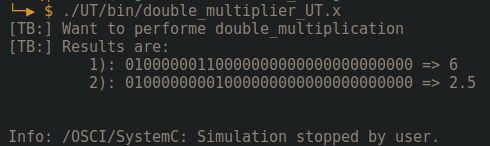
\includegraphics[width=\linewidth]{figures/SIM_TLM_UT.png}
    \caption{Simulazione con SystemC TLM untimed}
    \label{fig:SIM_TLM_UT}
\end{figure}
Nello stile \textbf{untimed} il testbench è l'initiator che chiama il target cioè il double\_multiplier, il quale elabora le moltiplicazioni e restituisce i risultati, sbloccando l'initiator. Nella figura \ref{fig:SIM_TLM_UT} si vedono i risultati ottenuti.

\begin{figure}[!htb]
    \centering
    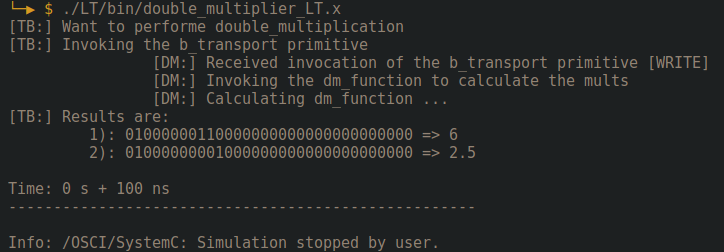
\includegraphics[width=\linewidth]{figures/SIM_TLM_LT.png}
    \caption{Simulazione con SystemC TLM loosely-timed}
    \label{fig:SIM_TLM_LT}
\end{figure}
Nello stile \textbf{loosely-timed}, analogamente all'untimed, il testbench chiama il double\_multiplier, il quale elabora le moltiplicazioni e restituisce i risultati con l'informazione di tempo trascorso. Come valore di \textbf{timing\_annotation} è stato utilizzato 100ns, valore ricavato dalla moltiplicazione di 10ns (cioè il periodo minimo a cui il componente sintezzato può funzionare) per 10 (cioè la lunghezza di cicli di clock media che sono necessari al componente per eseguire le due moltiplicazioni). Il numero di cicli di clock necessari all'esecuzione di una moltiplicazione può variare molto, come si può osservare lanciando la simulazione col \textbf{full\_target\_test} della descrizione in SystemC RTL. Come lunghezza del quanto per il loosely-timed è stato utilizzato il periodo di clock minimo cioè 10ns. Nella figura \ref{fig:SIM_TLM_UT} si vede bene che l'initiator invoca il target, resta in attesa della risposta e poi stampa i risultati. Si nota anche che dal tempo 0 sono passati 100ns.

\begin{figure}[!htb]
    \centering
    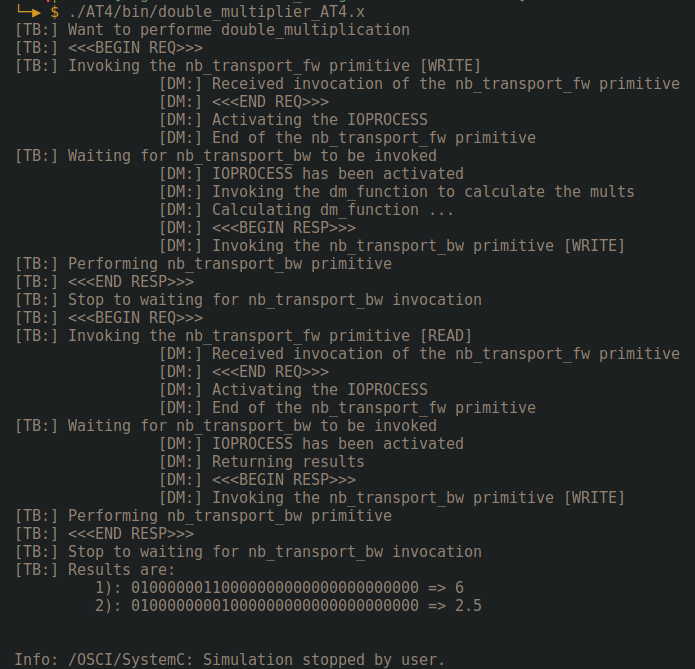
\includegraphics[width=\linewidth]{figures/SIM_TLM_AT4.png}
    \caption{Simulazione con SystemC TLM approximately-timed}
    \label{fig:SIM_TLM_AT4}
\end{figure}
Nello stile \textbf{approximately-timed} ci sono quattro fasi per la comunicazione osservabili in figura \ref{fig:SIM_TLM_AT4}:
\begin{itemize}
    \item Fase \textbf{BEGIN REQUEST}: l'initiator invoca il target, mandandogli gli operandi. Inizio forward-path
    \item Fase \textbf{END REQUEST}: il target riceve gli operandi e attiva IOPROCESS. Fine forward-path
    \item Fase \textbf{BEGIN RESPONSE}: vengono calcolate le moltiplicazioni e viene notificato l'initiato. Inizio backward-path
    \item Fase \textbf{END RESPONSE}: Viene ricevuta la notifica. Fine backward-paths
\end{itemize}
Analogamente si eseguendo le quattro fasi per ottenere il risultati.

\begin{figure}[!htb]
    \centering
    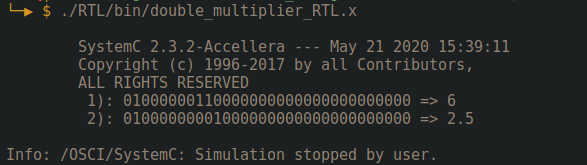
\includegraphics[width=\linewidth]{figures/SIM_RTL.png}
    \caption{Simulazione con SystemC RTL}
    \label{fig:SIM_RTL}
\end{figure}
Per rendere più significativo il confronto è stato riportato anche il progetto \textbf{RTL}, ma con con testbench analagoto a quello usato per gli stili del TLM. In figura \ref{fig:SIM_RTL} si vedono i risultati del test.
\\In ogni progetto SystemC, dentro il file ``define.hh'' si può attivare la modalità debug in cui viene testato il double\_multiplier con degli operandi scelti arbitrariamente e stampati dei messaggi per controllare il corretto funzionamento (figure \ref{fig:SIM_TLM_UT} \ref{fig:SIM_TLM_LT} \ref{fig:SIM_TLM_AT4} \ref{fig:SIM_RTL}). Se la modalità di debug è disattiva tutti i progetti eseguirano TESTNUM volte double\_multiplier con operandi generati randomicamente e non stamperanno nulla a video.
\\È stato poi messo a disposizione uno script dove è possibile eseguire con l'argomento:
\begin{itemize}
    \item \textbf{clean} il comando make clean in ogni directory, per eliminare i file sorgenti ed eseguibili.
    \item \textbf{make} il comando make in ogni directory, per eseguire la compilazione.
    \item \textbf{time} per eseguire sequenzialmente gli eseguibili con il comando \textit{time} per ricavare il tempo di esecuzione delle simulazioni.
\end{itemize}



\section{risultati}

\subsection{Simulazione e testbench sulla VirtualPlatform}
Il main del software legge un valore dal modulo I/O e chiama il driver di \textit{double\_multiplier} per eseguire la moltiplicazione con l'operando letto e altri 3 scelti arbitrariamente. Una volta ottenuto i risultati vengono poi trasmessi per essere letti in simulazione del testbench. (Nel main è anche presente la possibilità di utilizzare gli stessi operandi per eseguire due moltiplicazioni separate col driver \textit{float\_multiplier}).
\\Nel testbench scritto in verilog viene caricato il codice del software nella ROM, inviato un valore sul bus, che verrà poi utilizzato come operando e infine stampati i due risultati ottenuti. 
\\Nelle figure \ref{fig:SIM_VP} \ref{fig:SIM_VP_ZOOM} è possibile guardare la simulazione. In particolare si nota il corretto comportamento descritto in precedenza dalla EFSM (figura\ref{fig:EFSM_WRAPPER}) e il sequence diagram (figura\ref{fig:SEQ_DIAGRAM}) e l'elaborazione delle moltiplicazioni $1.0 \times  2.0 = 2.0$ e $3.0 \times 2.5 = 7.5$.

\subsection{TLM}

\begin{figure}[!htb]
    \centering
    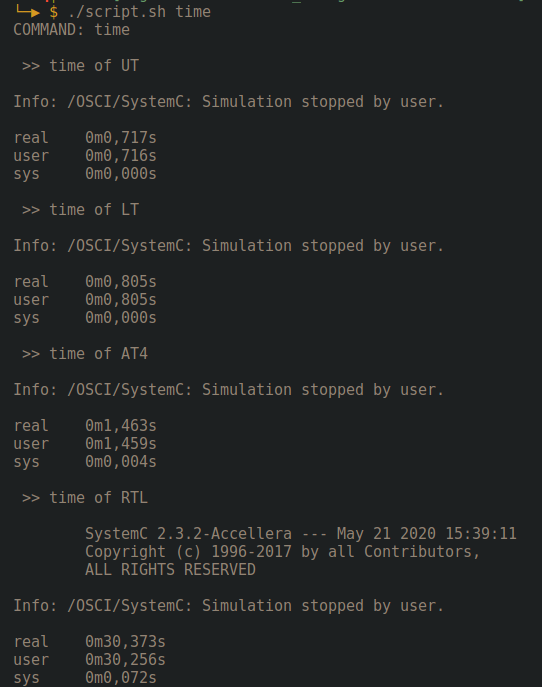
\includegraphics[width=0.9\linewidth]{figures/SIM_TLM_timing.png}
    \caption{Confronto timing simulazioni TLM e RTL con 1000000 esecuzioni di double\_multiplier}
    \label{fig:SIM_TLM_TIME}
\end{figure}
In figura \ref{fig:SIM_TLM_TIME} si vede che, come previsto, con l'aumentare dell'accuratezza temporale aumenta anche il tempo necessario per la simulazione. Si nota che fra lo stile untimed e loosely-timed non cambia molto, ma tra tra la versione più accurata TLM cioè approximately-timed e quella RTL c'è una grossa differenza.



\section{Conclusioni}
Sono rimasto particolarmente colpito dalla velocità delle simulazioni con SystemC-TLM rispetto a SystemC-RTL, ma soprattutto alla velocità con cui si riesce a scrivere il codice per descrivere il sistema funzionalmente. Purtroppo la versione approximately-timed risulta molto distante dalla versione RTL a livello di accuratezza, infatti viene usato un tempo medio di esecuzione del double\_multipler, il quale però varia molto in base agli operandi.
\\Sono soddisfatto dei risultati ottenuti e sicuramente questo progetto mi ha aiutato a comprendere meglio cos'è la progettazione basata su piattaforma e la sua utilità.



\nocite{*}
\bibliographystyle{IEEEtran}
\bibliography{biblio}
\appendix


\begin{figure*}[bt]
    \centering
    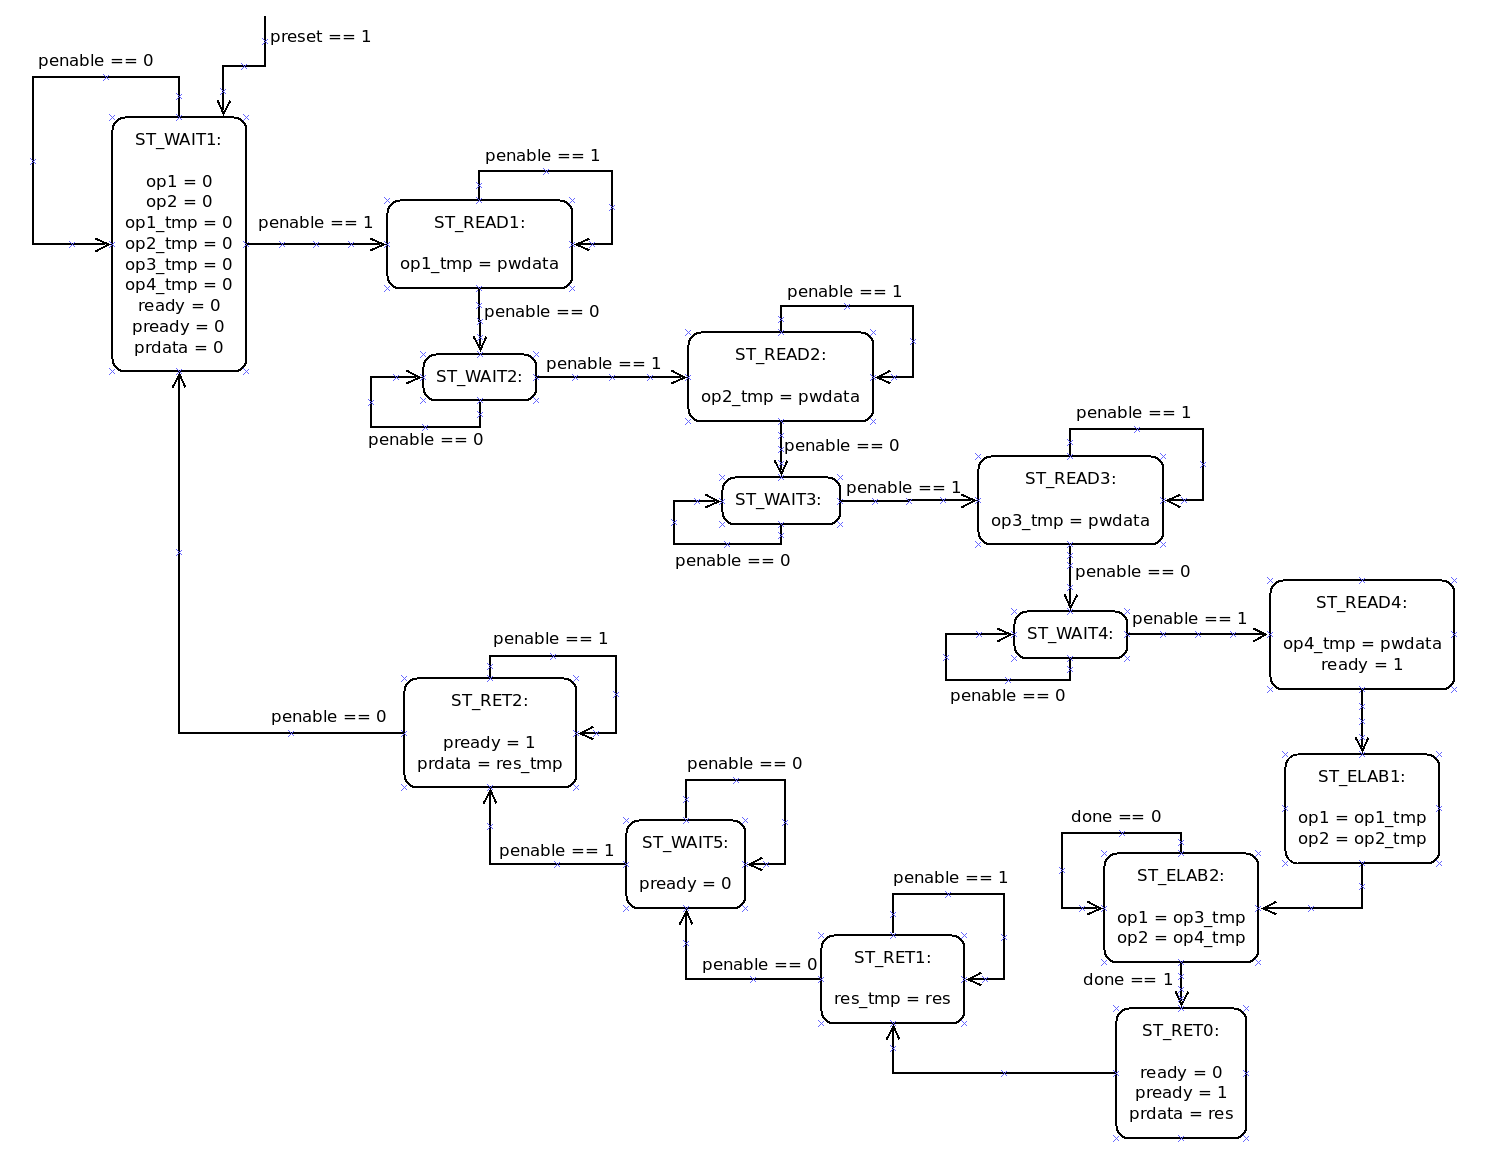
\includegraphics[width=\textwidth]{figures/EFSM_wrapper.png}
    \caption{EFSM del wrapper di double\_multiplier}
    \label{fig:EFSM_WRAPPER}
\end{figure*}

\begin{figure*}[bt]
    \centering
    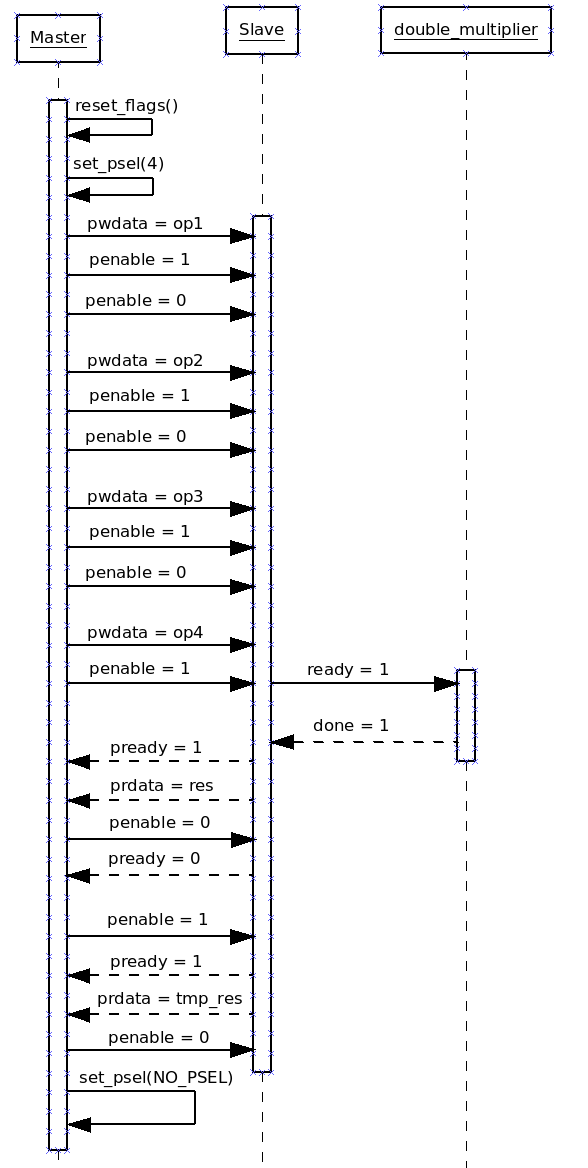
\includegraphics[width=0.5\textwidth]{figures/seq_diagram.png}
    \caption{Sequence diagram della comunicazione tra Master Slave e double\_multiplier}
    \label{fig:SEQ_DIAGRAM}
\end{figure*}

\begin{figure*}[bt]
    \centering
    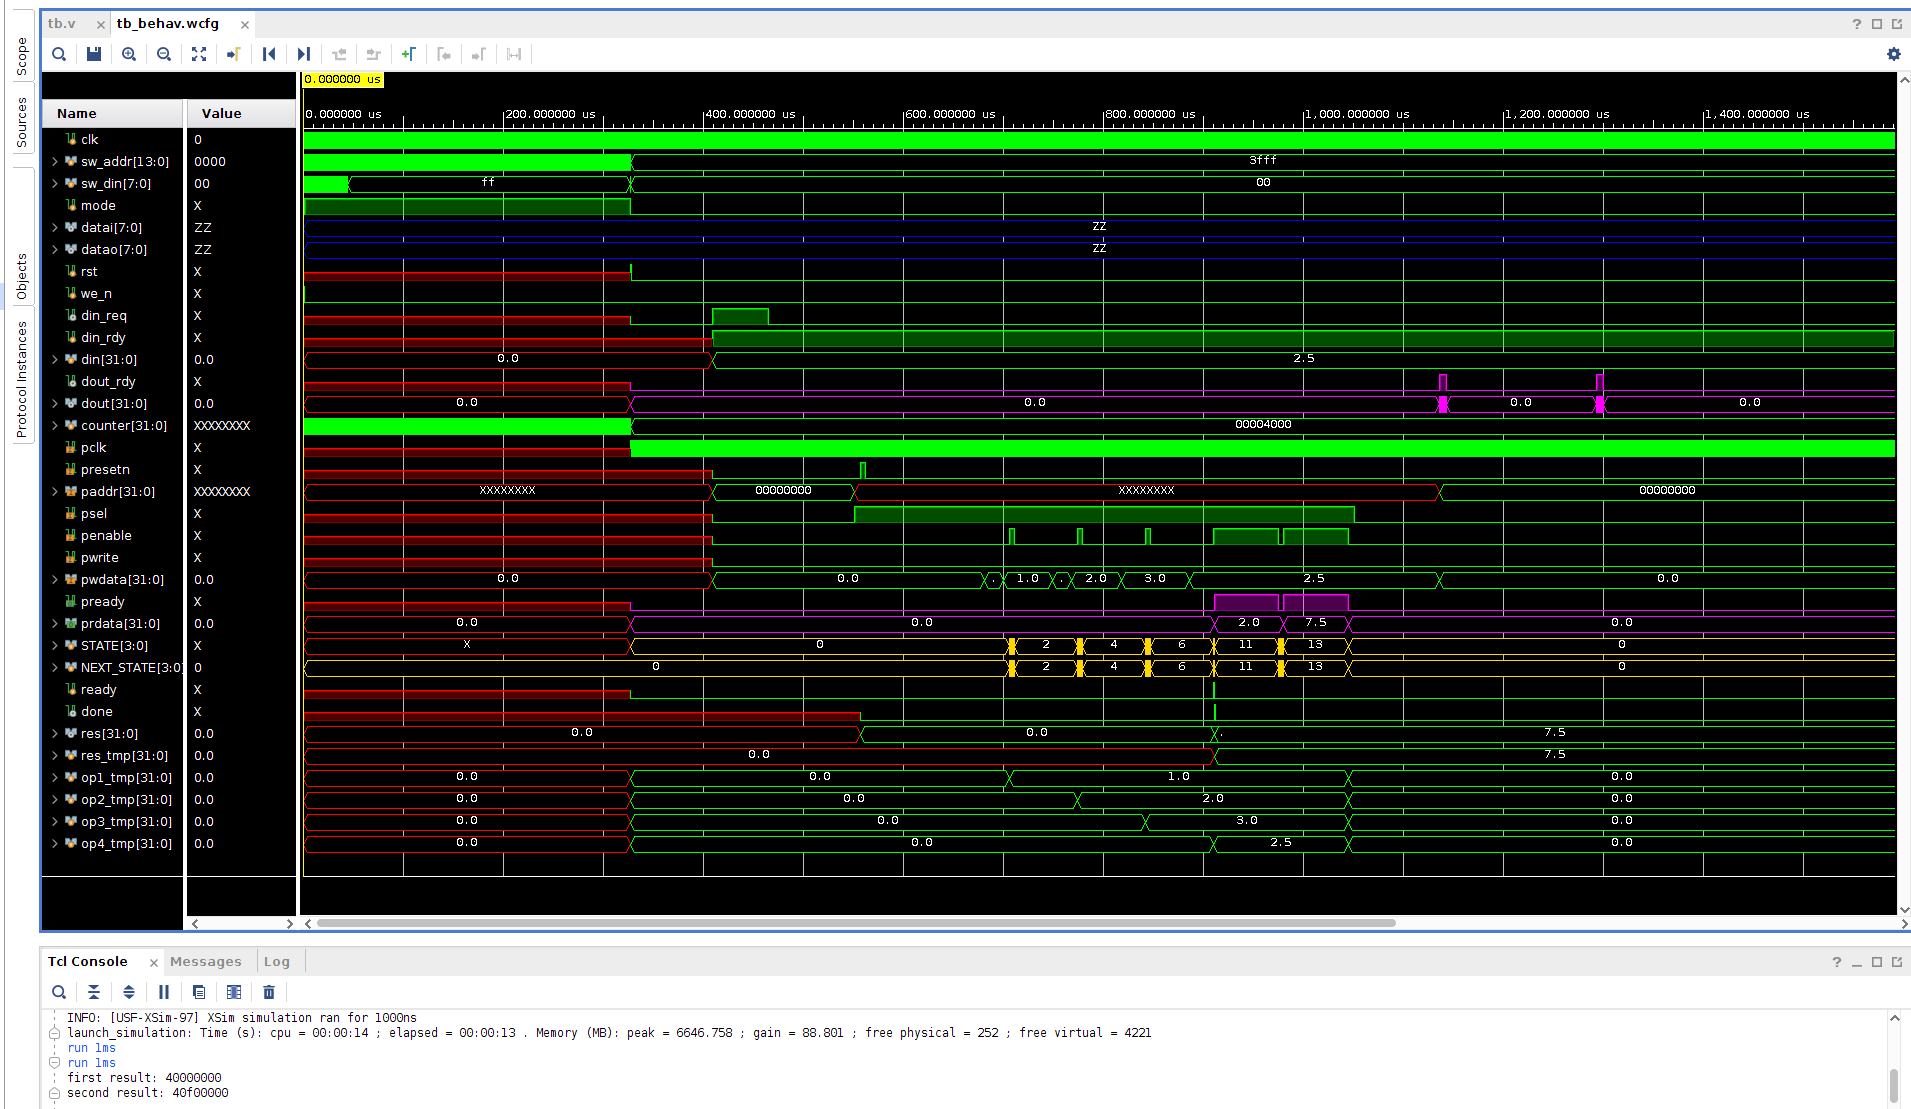
\includegraphics[width=\textwidth]{figures/SIM_VP.png}
    \caption{Simulazione virtual platform}
    \label{fig:SIM_VP}
\end{figure*}

\begin{figure*}[bt]
    \centering
    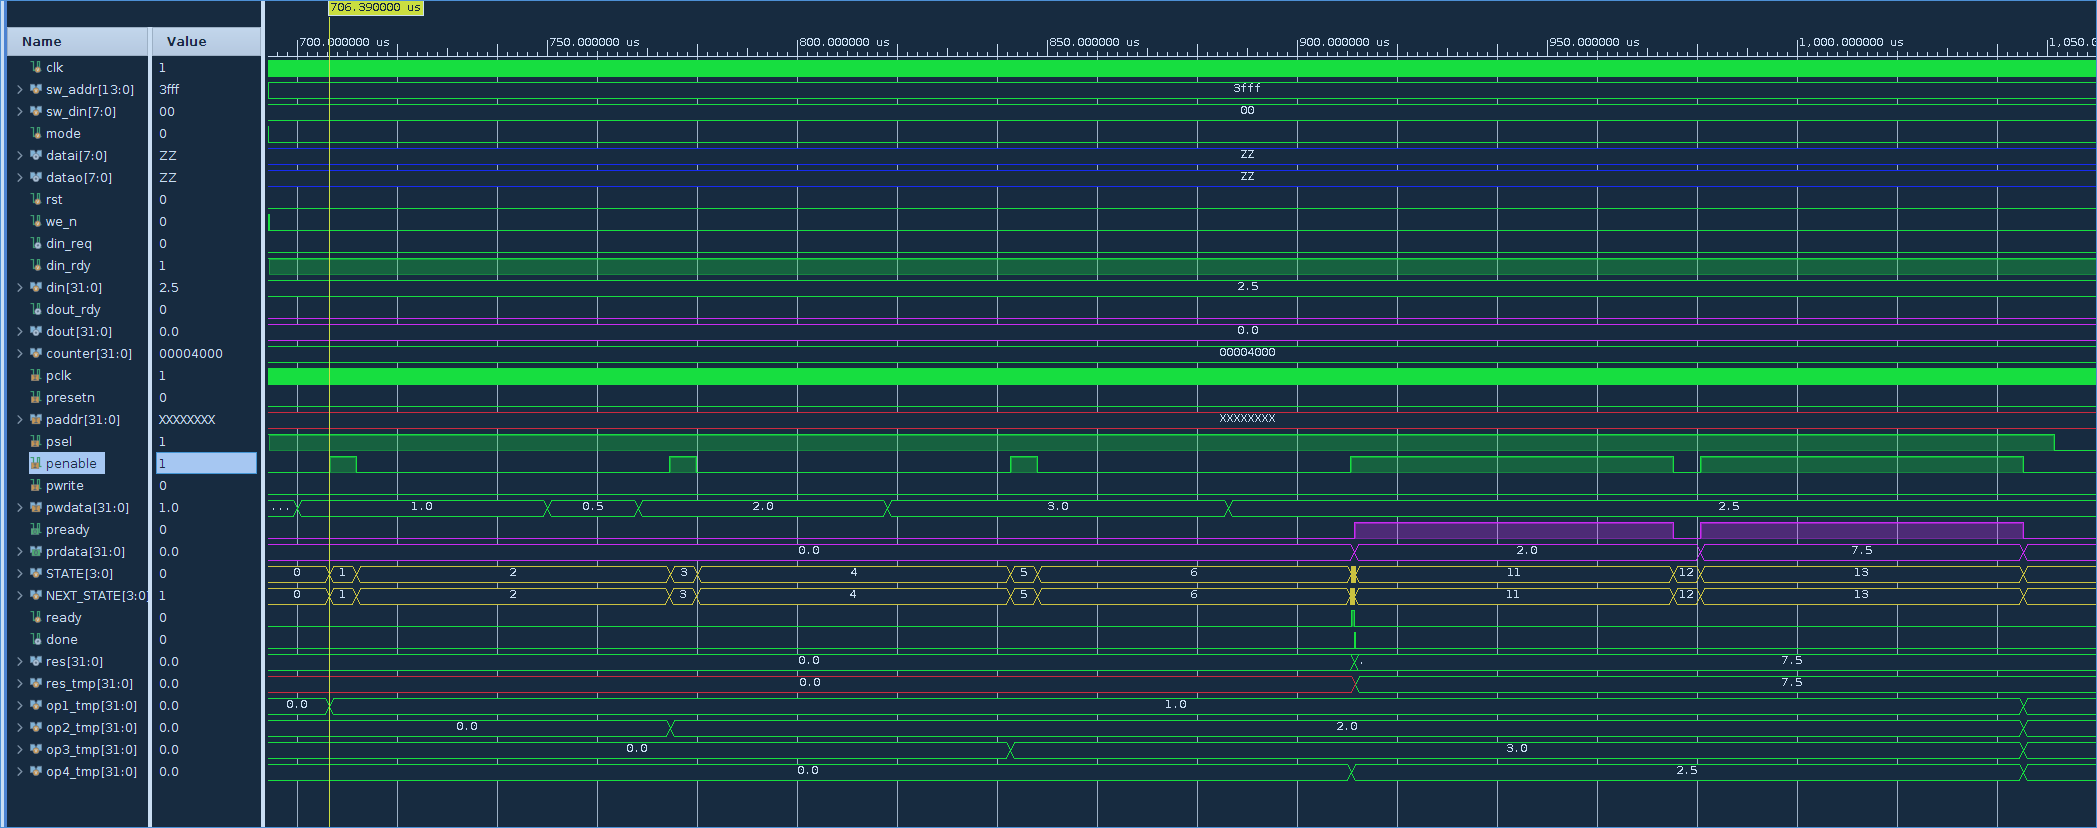
\includegraphics[width=\textwidth]{figures/SIM_VP_ZOOM.png}
    \caption{Simulazione con zoom virtual platform}
    \label{fig:SIM_VP_ZOOM}
\end{figure*}

\end{document}